\documentclass[tikz, crop, border=5pt]{standalone}
\usetikzlibrary{positioning,backgrounds,fit,shapes.geometric,calc}

\usepackage{fontspec}
\usepackage{xeCJK}

\setmainfont{NotoSans}[
    Extension      = .ttf,
    UprightFont    = *-Regular,
    BoldFont       = *-Bold,
    ItalicFont     = *-Italic,
    BoldItalicFont = *-BoldItalic
]

\usepackage{color}
\definecolor{module}{RGB}{188,36,46} % red

\tikzset{
    base/.style={
        draw=module,
        fill=module,
        text=white,
        font=\small,
    },
    % Adenylation
    A/.style={
        base,
        circle,
        minimum size=1cm,
        anchor=south,
        yshift=-2mm,
    },
    % Condensation
    C/.style={
        base,
        regular polygon,
        regular polygon sides=3,
        shape border rotate=180,
        minimum width=0.9cm,
        anchor=north,
    },
    % Epimerization
    E/.style={
        base,
        regular polygon,
        regular polygon sides=3,
        shape border rotate=0,
        minimum width=0.9cm,
        anchor=south,
    },
    % Condensation/Epimerization
    CE/.style={
        base,
        diamond,
        minimum width=0.8cm,
        minimum height=1.39cm,
    },
    % Thiolation
    T/.style={
        base,
        rectangle,
        minimum height=0.4cm,
        minimum width=0.2cm,
        anchor=north,
    },
    % Thioesterase
    Te/.style={
        base,
        circle,
        minimum width=0.7cm,
        anchor=north,
        yshift=2mm,
    },
    % Reductase
    R/.style={
        base,
        regular polygon,
        regular polygon sides=4,
        minimum width=0.8cm,
        anchor=north,
        yshift=2mm,
    },
    % Methyltransferase
    M/.style={
        base,
        ellipse,
        minimum width=0.9cm,
        minimum height=0.6cm,
    },
}

\begin{document}
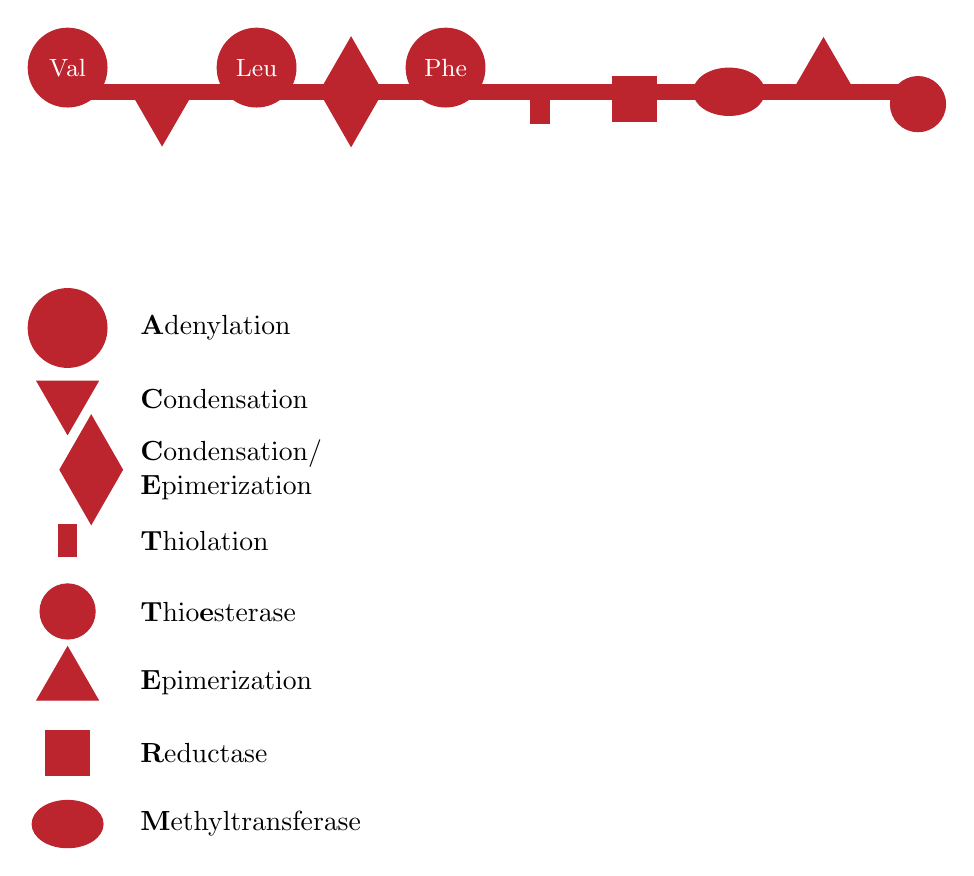
\begin{tikzpicture}
    % Draw module sequence
    \begin{scope}[on background layer]
        \draw[module, line width=2mm] (0,0) -- (10.8,0);
    \end{scope}

    \node[A] (A1) at (0,0) {Val};
    \node[C] (A2) at (1.2,0) {};
    \node[A] (A3) at (2.4,0) {Leu};
    \node[CE] (A4) at (3.6,0) {};
    \node[A] (A5) at (4.8,0) {Phe};
    \node[T] (A6) at (6.0,0) {};
    \node[R] (A7) at (7.2,0) {};
    \node[M] (A8) at (8.4,0) {};
    \node[E] (A9) at (9.6,0) {};
    \node[Te] (A10) at (10.8,0) {};

    % Legend
    \begin{scope}[yshift=-3cm]
        \begin{scope}[yshift=0cm]
            \node[A,anchor=center,yshift=2mm,] at (0,0) {};
            \node[anchor=west] at (0.8,0) {\textbf{A}denylation};
        \end{scope}

        \begin{scope}[yshift=-0.9cm]
            \node[C,anchor=center] at (0,0) {};
            \node[anchor=west] at (0.8,0) {\textbf{C}ondensation};
        \end{scope}

        \begin{scope}[yshift=-1.8cm]
            \node[CE] at (0.3,0) {};
            \node[anchor=west,align=left] at (0.8,0) {\textbf{C}ondensation/\\\textbf{E}pimerization};
        \end{scope}

        \begin{scope}[yshift=-2.7cm]
            \node[T,anchor=center] at (0,0) {};
            \node[anchor=west] at (0.8,0) {\textbf{T}hiolation};
        \end{scope}

        \begin{scope}[yshift=-3.6cm]
            \node[Te,anchor=center,yshift=-2mm,] at (0,0) {};
            \node[anchor=west] at (0.8,0) {\textbf{T}hio\textbf{e}sterase};
        \end{scope}

        \begin{scope}[yshift=-4.5cm]
            \node[E,anchor=center] at (0,0) {};
            \node[anchor=west] at (0.8,0) {\textbf{E}pimerization};
        \end{scope}

        \begin{scope}[yshift=-5.4cm]
            \node[R,anchor=center,yshift=-2mm] at (0,0) {};
            \node[anchor=west] at (0.8,0) {\textbf{R}eductase};
        \end{scope}

        \begin{scope}[yshift=-6.3cm]
            \node[M] at (0,0) {};
            \node[anchor=west] at (0.8,0) {\textbf{M}ethyltransferase};
        \end{scope}
    \end{scope}
\end{tikzpicture}
\end{document}
